\documentclass[10pt,a4paper]{article}
%\usepackage[table]{xcolor}
%\usepackage{float}
\usepackage[spanish]{babel}
\usepackage{amsmath}
%\usepackage{amssymb}
\usepackage{graphicx}
%\usepackage{amsfonts}
\usepackage[utf8]{inputenx}
\usepackage{pdfpages}
\usepackage{listings}
%\usepackage{algorithm2e}
%\usepackage{listings}
%\usepackage{pdfpages}
%\usepackage{tabularx}
%\usepackage{color}
\usepackage{anysize}
\usepackage{fancyhdr}
\usepackage{ulem}
\usepackage{hyperref}
%\usepackage{caption}
\usepackage[font=footnotesize]{caption}
\definecolor{deepblue}{RGB}{0,0,153}
\definecolor{deepred}{RGB}{153,0,0}
\definecolor{deepgreen}{RGB}{51,102,0}
\definecolor{deepyellow}{RGB}{204,204,0}
\marginsize{2cm}{2cm}{1cm}{1.5cm} % depende de anysize
%\renewcommand*{\thefootnote}{\Roman{footnote}}
%\usepackage{hyperref}
%\hypersetup{
%    colorlinks=true,
%    citecolor=black,
%    filecolor=black,
%    linkcolor=black,
%    urlcolor=black,
%    linktoc=all
%}



%\title{Multímetros en Corriente Continua}
\title{Universidad de Buenos Aires - FIUBA \\
		66.20 Organización de Computadoras \\
		Trabajo Práctico 0: Infraestructura Básica\\}
\author{	Joaquin Segui, \textit{Padrón Nro. 91.451}                     \\
            \texttt{ segui.joaquin@gmail.com }                                          \\[2.5ex]
            Pernin Alejandro, \textit{Padrón Nro. 92.216}                     \\
            \texttt{ale.pernin@gmail.com}                                              \\[2.5ex]
            Menniti Sebastián Ezequiel, \textit{Padrón Nro. 93.445}                     \\
            \texttt{ mennitise@gmail.com }                                              \\[2.5ex]}
\date{}

%\lfoot{asdasd}


\begin{document}
%\includepdf{attachments/caratula.pdf}


%\newpage\null\thispagestyle{empty}\newpage
\maketitle\thispagestyle{empty}

\newpage\null\thispagestyle{empty}\newpage

%\newpage
%\tableofcontents

%\newpage\null\thispagestyle{empty}\newpage

\section{Introducción}

Se implemento un programa, en lenguaje C, que se encarga de multiplicar matrices de números reales, representados en punto flotante de doble precisión.


\section{Diseño e Implementación}

Las matrices a multiplicar se ingresan por entrada estándar (\texttt{stdin}), donde cada linea representada una matríz completa en formato de texto, describiendola mediante el siguiente formato:

\begin{center}

$NxM \: a_{1,1} \: a_{1,2} \: ... \: a_{1,M} \: a_{2,1} \: a_{2,2} \: ... \: a_{2,M} \: ... \: a_{N,1} \: a_{N,2} \: ... \: a_{N,M}$

\end{center}
Esta linea representa a una matríz \textit{A}, donde \textit{N} es la cantidad de filas y \textit{M} la cantidad de columnas de la matríz \textit{A}. Los elementos de la matríz \textit{A} son los \textit{$a_{x,y}$} , donde \textit{x} e \textit{y} son los indices de fila y columna respectivamente. El fin de linea se delimita con el caracter \textit{newline}.

Por cada par de matrices que se presentan en la entrada, el programa en primer lugar, se encarga de cargarlas, luego verifica que las matrices cumplan con la condición para que la multiplicación sea posible (Se verifica que la cantidad de columnas de la primer matríz sea igual a la cantidad de filas de la segunda matríz), y en el caso que la cumplan, se procede a multiplicarlas. El resultado obtenido lo presenta por salida estándar (\texttt{stdout}), en el mismo formato mencionado anteriormente. Este proceso se repite hasta que llegue al final del archivo de entrada (\texttt{EOF}). Si se encontrara con un error, el programa lo informa por \texttt{stderr} y se detiene su ejecución.



\section{Comandos para compilar el programa}
Para facilitar la compilacion se utiliza un \textit{Makefile}, para invocar la compilación del programa ejecutar desde una consola, dentro del mismo directorio que el código fuente: \texttt{make}.

Asimismo se proviciona un script que realiza pruebas con un set de datos preexistente, para invocarlo: \texttt{./pruebas.sh}.

\section{Pruebas}
	En esta sección se detallarán las pruebas realizadas. Los archivos utilizados se encuentran el el directorio \textit{test\_files}.
	\subsection{Casos Exitosos}
		Los casos exitosos están comprendidos por los set de datos \textit{test1} y \	textit{test2}.	
		En el caso del	 primero:\	
	
		\lstinputlisting[basicstyle=\footnotesize]{../src/test_files/test1.txt}
	
		Representa la operación
		\begin{center}
		$\begin{pmatrix}
		1 & 2
		\end{pmatrix}
		*
		\begin{pmatrix}
		1 & 0 & 4 \\ 5 & 1 & 3
		\end{pmatrix}
		=
		\begin{pmatrix}
		11 & 2 & 10
		\end{pmatrix}
		$
		\end{center}
	
		cuya salida por consola mediante el script de pruebas es
	
		\texttt{1x3 11 2 10 }
	
		como es esperable.\\
	
		El segundo set de datos es:
		\lstinputlisting[basicstyle=\footnotesize]{../src/test_files/test2.txt}
	
		representando las operaciones
	
		\begin{center}
		$\begin{pmatrix}
		1 \\ 2 \\ 3
		\end{pmatrix}
		*
		\begin{pmatrix}
		0 & 3 & 1
		\end{pmatrix}
		=
		\begin{pmatrix}
		0 & 3 & 1 \\ 0 & 6 & 2 \\ 0 & 9 & 3
		\end{pmatrix}
		$\end{center}
	
		\begin{center}
		$\begin{pmatrix}
		1 & 3
		\end{pmatrix}
		*
		\begin{pmatrix}
		1 & 0 & 4 \\ 5 & 1 & 0
		\end{pmatrix}
		=
		\begin{pmatrix}
		16 & 3 & 4
		\end{pmatrix}
		$\end{center}
	
		cuya salida se obtuvo correctamente
	
		\texttt{3x3 0 3 1 0 6 2 0 9 3}

		\texttt{1x3 16 3 4}

	\subsection{Casos de error}
		Como casos de error del programa probamos matrices incompatibles para su multiplicacion y matrices mal definidas.

		Uno de estos casos es el de tener dos matrices cuyas dimensiones hacen incompatibles la multiplicación entre sí. Este es el caso del set \textit{test3}.

		\lstinputlisting[basicstyle=\footnotesize]{../src/test_files/test3.txt}
		\begin{center}
		$\begin{pmatrix}
		1 & 2
		\end{pmatrix}
		*
		\begin{pmatrix}
		1 & 0 & 4
		\end{pmatrix}
		$\end{center}

		Al ejecutar dicha prueba, el programa termina con el siguiente mensaje:

		\texttt{Dimensiones no compatibles para multiplicar}\\

		Otra prueba es tener una cantidad impar de matrices, por lo cuál una no podrá ser multiplicada. Por ejemplo \textit{test4}.

		\lstinputlisting[basicstyle=\footnotesize]{../src/test_files/test4.txt}
		
		Como resultado arroja

		\texttt{3x3 0 3 1 0 6 2 0 9 3}

		\texttt{Fallo al leer dimensiones}\\

		Otros casos de prueba, consisten en definir dimensiones de matrices inconsistentes con la cantidad de elementos leidos. Al ver \textit{test5}

		\lstinputlisting[basicstyle=\footnotesize]{../src/test_files/test5.txt}

		\begin{center}
		$\begin{pmatrix}
		1 \\ 2 \\ X
		\end{pmatrix}
		*
		\begin{pmatrix}
		0 & 3 & 1
		\end{pmatrix}
		$\end{center}

		si bien las dimensiones declaradas son compatibles para su multiplicación, los elementos provistos son inconsistentes. Dicha prueba arroja:

		\texttt{Cantidad elementos distinta a dimensiones de matriz}


\newpage
\section{Codigo fuente del programa}

\subsection{En lenguaje C}

\lstinputlisting[
			language=C,
			basicstyle=\footnotesize,
			numbers=left,
			stepnumber=1,
			numbersep=4pt,
			tabsize=2,
			otherkeywords={self}, 
			keywordstyle=\color{deepred},
			stringstyle=\color{deepgreen},
			commentstyle=\color{deepblue},
			]{../src/main.c}

\newpage
\subsection{Codigo MIPS32 generado por el compilador}

\lstinputlisting[
			language=Assembler,
			basicstyle=\footnotesize,
			numbers=left,
			stepnumber=1,
			numbersep=4pt,
			tabsize=2,
			otherkeywords={self}, 
			keywordstyle=\color{deepred},
			stringstyle=\color{deepgreen},
			commentstyle=\color{deepblue},
			]{../src/main.s}
}
\newpage\thispagestyle{empty}
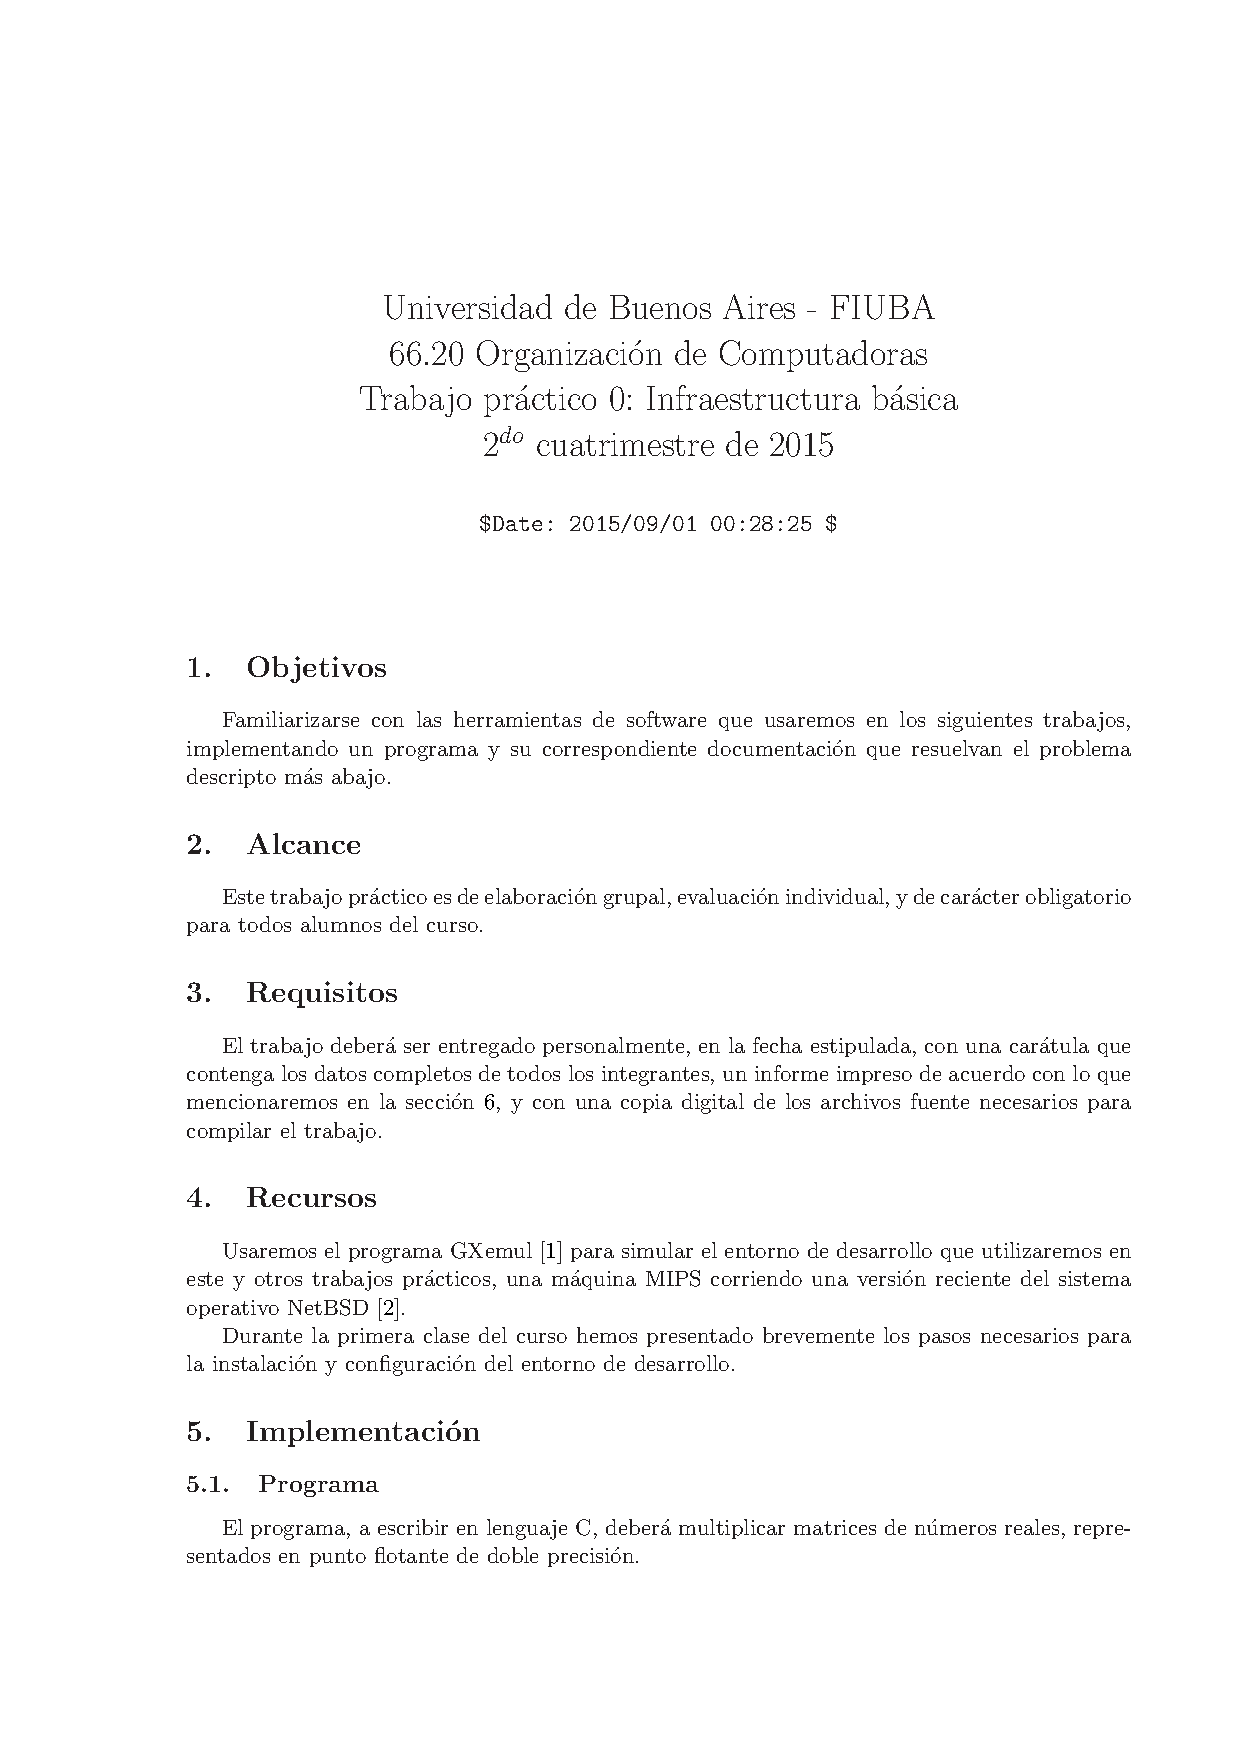
\includepdf[pages=1,pagecommand=\subsection{Enunciado}]{tp0-2015-2q.pdf}
\includepdf[pages=2-,]{tp0-2015-2q.pdf}

\end{document}